\section{INTRODUCCIÓN} \label{sec:introduccion}

\subsection{Justificación}

Actualmente, el mundo atraviesa una crisis energética global desencadenada en el año 2021 principalmente por la recuperación económica tras la pandemia y agravada tras la invasión rusa de Ucrania en febrero de 2022. El precio del gas natural alcanzó máximos históricos, aumentando consecuentemente en muchos casos el coste de la electricidad en general. Familias, empresas e industrias se han visto gravemente afectadas, llevando a diversos países en camino de una fuerte recesión económica. Consecuentemente, la reducción de los costes energéticos se convierte en una de las principales prioridades de empresas y ciudadanos, y la independencia energética, la
garantía de suministro y la lucha contra el cambio climático adquieren una gran importancia en el debate público de gran cantidad de países (\cite{crisis_energetica_iea}). 

Frente a esta situación, la energía nuclear está tomando cada vez más relevancia en muchos países, considerándose un factor clave para conseguir los grandes desafíos políticos, económicos y climáticos  a los que se enfrenta la sociedad actual en un escenario tan complicado. Numerosos países han optado por ampliar su parque nuclear existente, muchos han decidido alargar la vida de sus reactores nucleares actualmente en operación y algunos han comenzado a construir sus primeras centrales nucleares. 

\begin{table}[h]
    \resizebox{\textwidth}{!}{%
    \begin{tabular}{|cc|cc|cc|}
    \hline
    \rowcolor[HTML]{ECF4FF} 
    \multicolumn{2}{|l|}{\cellcolor[HTML]{ECF4FF}\textbf{Generación de electricidad nuclear}} &
      \multicolumn{2}{l|}{\cellcolor[HTML]{ECF4FF}\textbf{Reactores en operación}\tablefootnote{\textbf{En operación:} Conectados a la red.}} &
      \multicolumn{2}{l|}{\cellcolor[HTML]{ECF4FF}\textbf{Reactores en construcción}\tablefootnote{\textbf{En construcción:} primer hormigón vertido para el reactor.}} \\ \hline
    \rowcolor[HTML]{FFFFFF} 
    \multicolumn{1}{|c|}{\cellcolor[HTML]{FFFFFF}\textbf{9,8}} &
      2.808 TWh &
      \multicolumn{1}{c|}{\cellcolor[HTML]{FFFFFF}\textbf{436}} &
      392.114 MWe &
      \multicolumn{1}{c|}{\cellcolor[HTML]{FFFFFF}{\color[HTML]{000000} \textbf{62}}} &
      {\color[HTML]{000000} 69.279 MWe} \\ \hline
    \rowcolor[HTML]{ECF4FF} 
    \multicolumn{2}{|c|}{\cellcolor[HTML]{ECF4FF}\textbf{Reactores planificados}\tablefootnote{\textbf{Planificados:} Aprobaciones, financiamiento o compromiso en vigor. Se espera que estén en funcionamiento en los próximos 15 años.}} &
      \multicolumn{2}{c|}{\cellcolor[HTML]{ECF4FF}\textbf{Reactores propuestos}\tablefootnote{\textbf{Propuestos:} Programa específico o propuestas de sitio; tiempo muy incierto.}} &
      \multicolumn{2}{c|}{\cellcolor[HTML]{ECF4FF}\textbf{OLP aprobada}\tablefootnote{\textbf{\acrfull{olp} aprobada:} Autorización a operar más allá de los 40 años. En Estados Unidos, la mayoría de reactores tiene licencia para operar a 60 años y 6 tienen permiso para operar hasta los 80.}} \\ \hline
    \multicolumn{1}{|c|}{\cellcolor[HTML]{FFFFFF}\textbf{110}} &
      \cellcolor[HTML]{FFFFFF}112.877 MWe &
      \multicolumn{1}{c|}{\cellcolor[HTML]{FFFFFF}\textbf{333}} &
      \cellcolor[HTML]{FFFFFF}366.652 MWe &
      \multicolumn{2}{c|}{\textbf{191}} \\ \hline
    \end{tabular}%
    }
    \caption{Resumen de la situación actual de la energía nuclear en el mundo (\cite{world_nuclear_power_reactors}).}
    \label{tab:situacion_nuclear_mundial}
    \end{table}

    \begin{wrapfigure}{r}{0.52\textwidth}
      \vspace{-0.5cm}
      \centering
      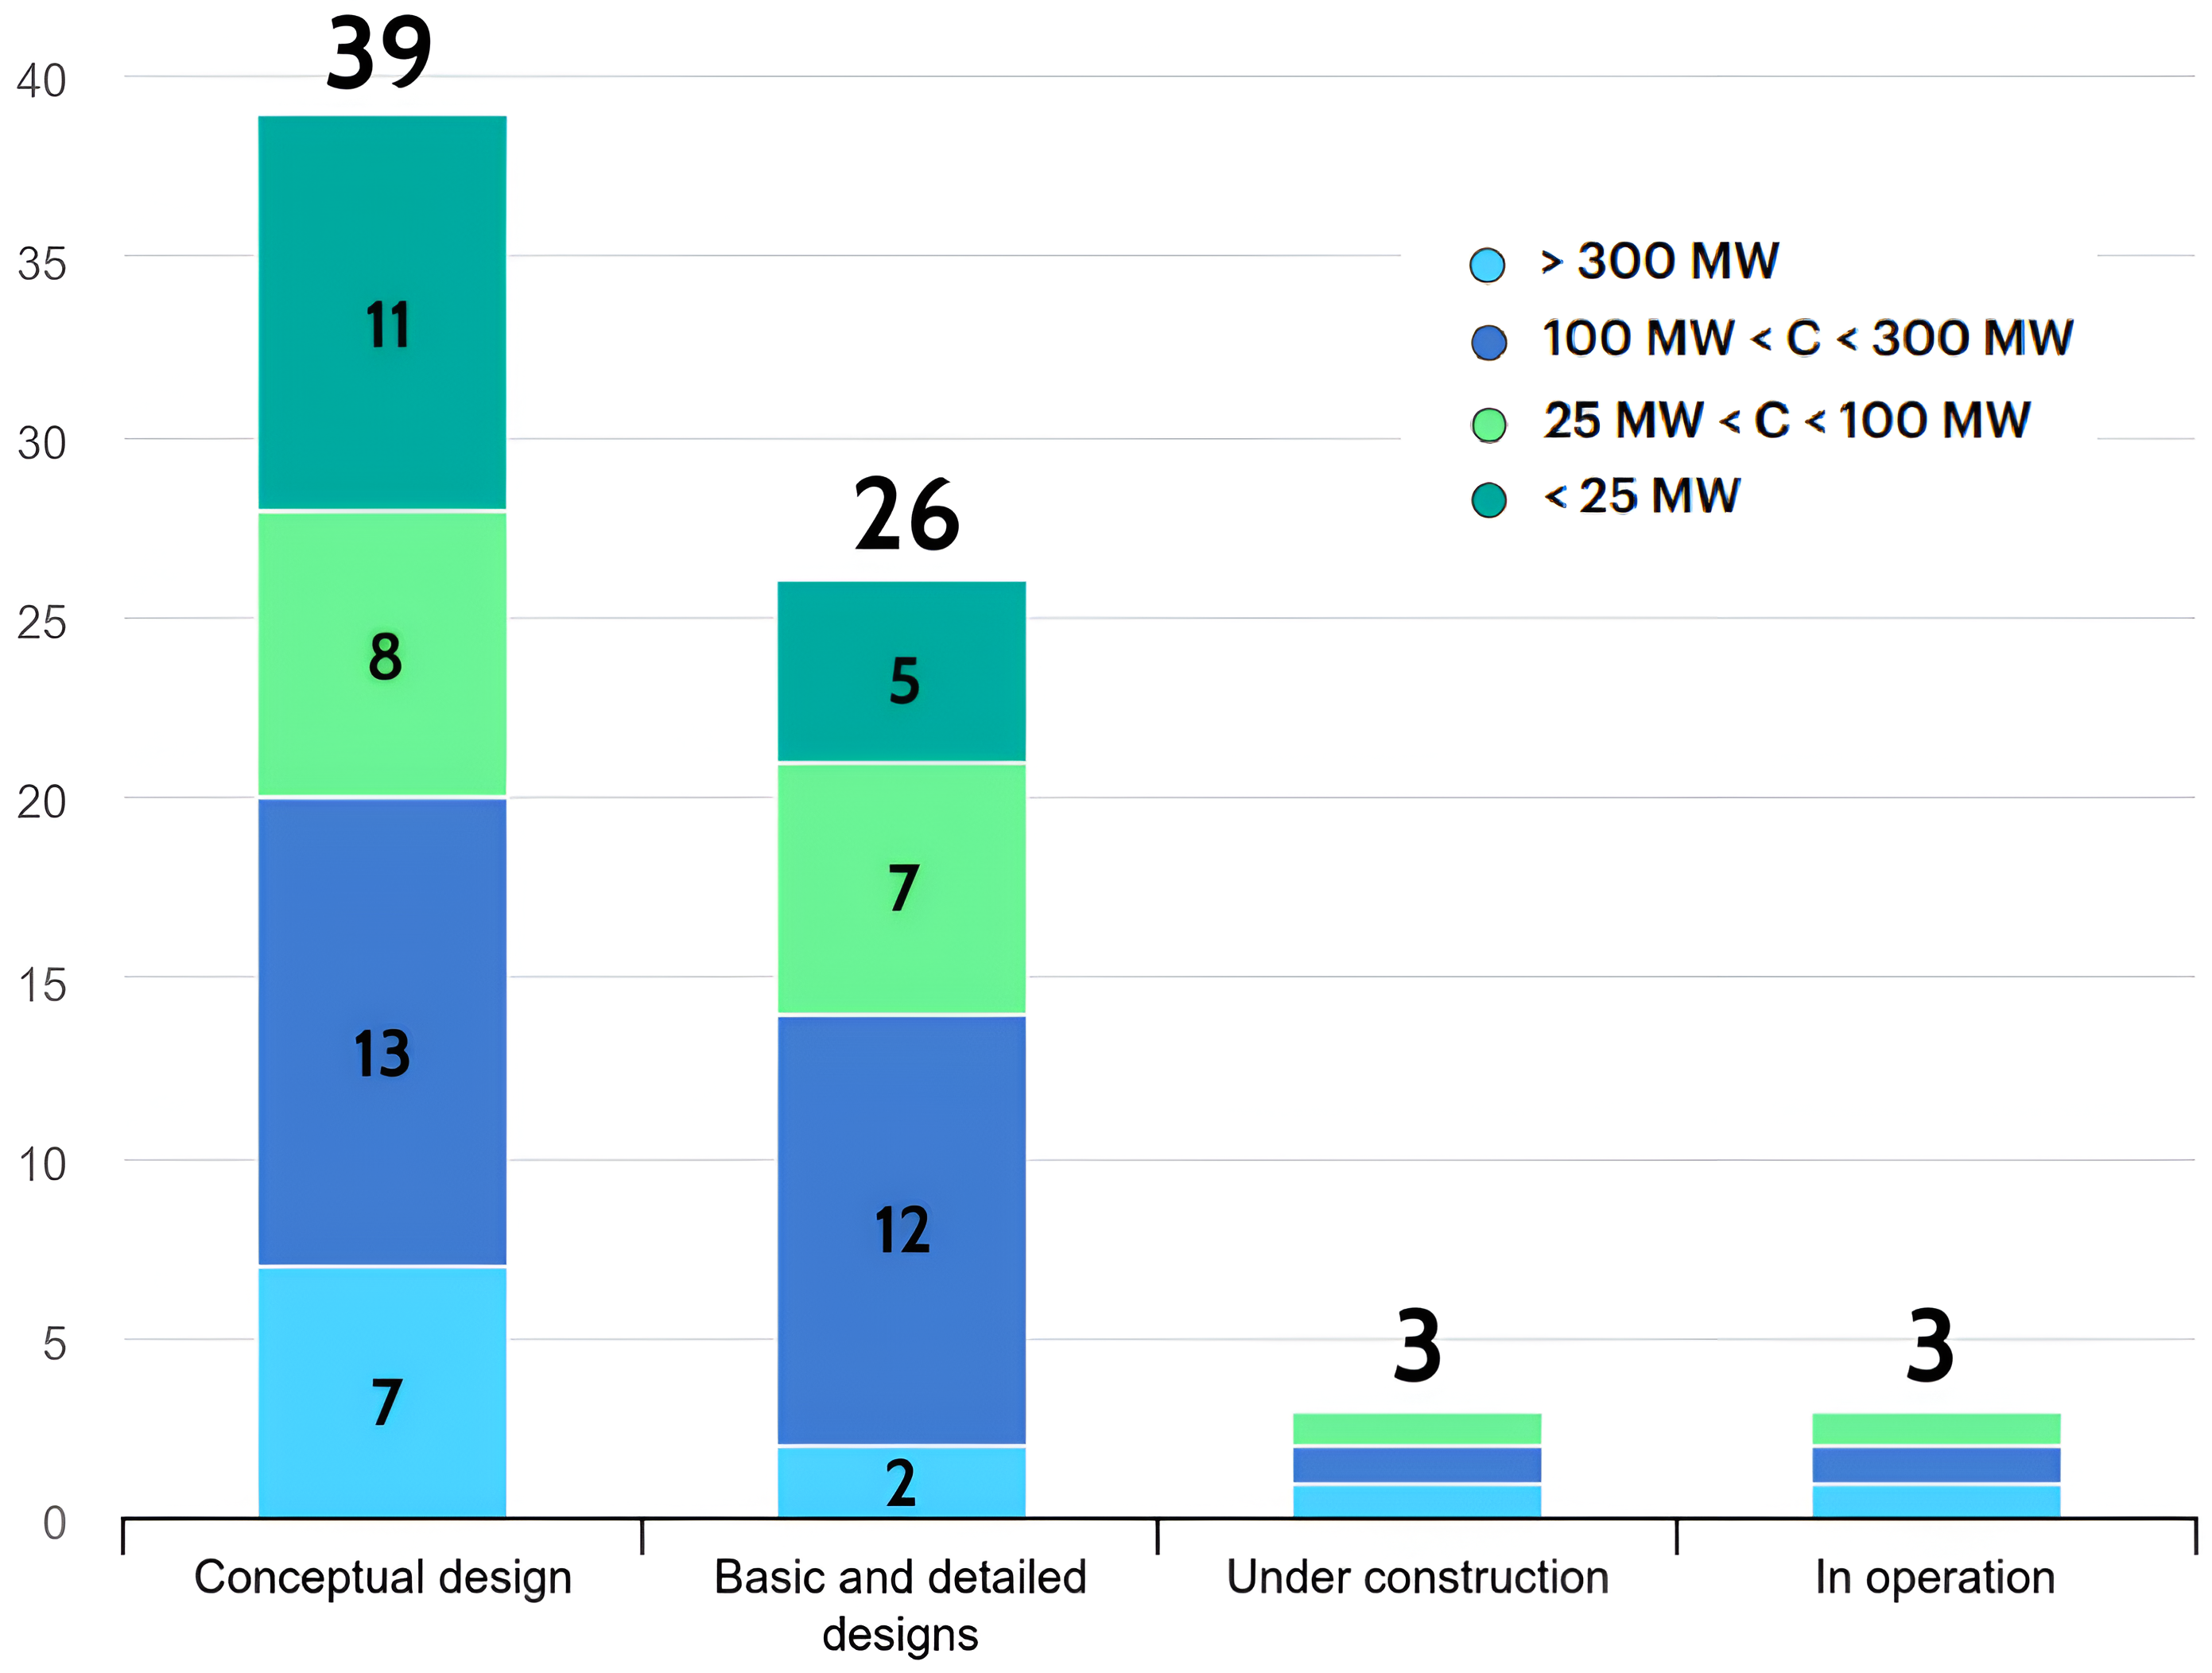
\includegraphics[width=0.52\textwidth]{content/figures/global_smr_projects2.png}
      \caption{\acrshortpl{smr} en el mundo (\cite{iea_global_smr_projects}).}
      \label{fig:global_smr_projects}
      \vspace{-1cm}
    \end{wrapfigure}

    En este contexto, se ha incrementado muy considerablemente el interés por los reactores modulares pequeños, ampliamente conocidos como \emph{\acrfullpl{smr}}. Se trata de una tecnología avanzada de menor escala que la convencional que ofrece grandes ventajas en lo que a coste, tiempo de construcción, seguridad y versatilidad se refiere. Por consiguiente, múltiples instituciones públicas y privadas están participando activamente en los esfuerzos encaminados a hacer prosperar esta tecnología, existiendo más de 80 diseños de \acrshortpl{smr} comerciales que se están desarrollando en todo el mundo (\cite{smr_oiea}).




    
\newpage 

Este creciente empuje de la industria nuclear está contribuyendo a un aumento de profesionales especializados en este sector y, paralelamente, a una creciente necesidad de futuros profesionales nucleares. En este contexto y frente a los grandes avances tecnológicos desarrollados actualmente, cobran una especial importancia los \textbf{simuladores} empleados tanto en el ámbito del análisis numérico como en la formación de operadores, técnicos e ingenieros nucleares. Existen múltiples simuladores virtuales y físicos desarrollados por diversas instituciones y empresas que permiten enfrentarse a las condiciones de operación, maniobras y accidentes que pueden suceder en una central nuclear. La Escuela Técnica Superior de Ingenieros Industriales de Madrid (ETSII - UPM) tiene a su disposición el \acrfull{sgiz}, con el cual se trabajará en el presente proyecto para profundizar en el estudio de la operación de las centrales nucleares y, en concreto, en la operación de un \acrshort{smr}, debido a las grandes similitudes que el simulador en cuestión presenta con respecto a esta innovadora tecnología.

\subsection{Objetivos}

El principal objetivo de este trabajo fin de grado es \textbf{simular maniobras de seguimiento de carga de una central nuclear muy similar a un \acrshort{smr}} mediante el \acrshort{sgiz} de la Escuela. Este tipo de maniobras es una de las aplicaciones fundamentales para las que se concibe el diseño de los \acrshortpl{smr} y presentan un gran interés actualmente. Para ello, y como segundo objetivo fundamental, se pretende \textbf{conocer en profundidad el funcionamiento de un \acrshort{smr}; sus sistemas de seguridad, protección y control, y su modo de operación}.

Asimismo, existen paralelamente diversos objetivos secundarios. En primer lugar, familiarizarse con el tipo de software empleado en los simuladores del ámbito nuclear. En segundo lugar, conocer el estado del arte, las características, las grandes ventajas y los desafíos de la tecnología de los \acrshortpl{smr}. Por último, implementar las simulaciones realizadas al programa de prácticas de la asignatura de Tecnologías Avanzadas en Reactores Nucleares del Máster en Ciencia y Tecnología Nuclear impartido en la ETSII.

\subsection{Metodología}

El desarrollo de este proyecto parte de una adquisición completa de diversos conceptos teóricos que permitirán posteriormente focalizarse en la realización de simulaciones prácticas. Al mismo tiempo, estas simulaciones complementarán y consolidarán los conocimientos previos adquiridos y posibilitarán un aprendizaje en profundidad. De esta manera, el trabajo se fundamenta, en tres grandes bloques:

\begin{itemize}
  \item \textbf{Los \acrlongpl{smr}:} Comenzando por los orígenes de esta tecnología, posteriormente se analizan detalladamente las ventajas que presenta frente a los reactores de gran escala y se clasifican los distintos tipos de pequeños reactores modulares existentes. Por último, se analiza un \acrshort{smr} en concreto ---el AP300--- por su similitud con el reactor del simulador con el que se trabaja ---el \acrshort{sgiz}---.
  \item \textbf{Los simuladores:} En primer lugar, se clasifican los distintos tipos de simuladores existentes en función de los objetivos, las ventajas y las funcionalidades que presentan. En segundo lugar, se analizan casos concretos de simuladores de \acrshortpl{smr} para conocer el estado del arte de este tipo de simulación. Seguidamente, se detallan las ventajas del empleo de simuladores para fines formativos y didácticos. Por último, se estudia la Central Nuclear de Zorita, a la cual pertenece el \acrshort{sgiz}, comparándola con el AP300 para ver su parecido con un \acrshort{smr}. Además, se finaliza este estudio con una descripción de las características y modos de operación del \acrshort{sgiz}.
  \item \textbf{Las simulaciones:} Como el proyecto se centra en el análisis de las capacidades de seguimiento de carga de los \acrshortpl{smr}, se comienza este apartado práctico con un estudio de este tipo de maniobras de variación de potencia en función de distintas necesidades. Seguidamente, se realizan múltiples simulaciones que, tras ser debidamente analizadas, permiten comprender en profundidad, no solo el seguimiento de carga, sino también el funcionamiento y los  sistemas más importantes de una central nuclear. En este bloque se incluye la implementación de una de las simulaciones como práctica académica.
\end{itemize}